\section{Erster Commit}
\begin{lstlisting}
$ git add README.md
$ git status
On branch master

No commits yet

Changes to be committed:
  (use "git rm --cached <file>..." to unstage)
        new file:   README.md
\end{lstlisting}
An dieser Stelle wurde die Datei
\inline{README.md} dem nächsten Commit hinzugefügt. Um den Aktuellen Status zu protokollieren muss der Befehl \inline{git commit} genutzt werden. Dabei werden alle Änderungen Protokolliert.
Git speichert intern die Version der Datei ab und verweißt in jedem folge Commit darauf. Wenn die Datei nicht verändert wird wird somit nicht mehr Speicherplatz verwendet, egal in wie vielen Commits die Datei vorkommt.
Ein commit wird immer mit einer Commit-Message begleitet. Wenn der Befehl \inline{git commit} ohne Optionen ausgeführt wird öffnet sich daher automatisch der standard editor (der über \inline{git config --local core.editor} definiert wurde). In diesem Befindet sich eine auskommentierte Übersicht des Commits. Darunter muss eine Commit-Message eingefügt werden.
\begin{figure}[!h]
        \centering
        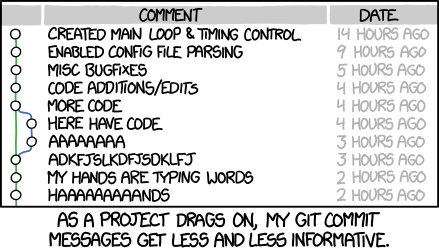
\includegraphics[width=0.5\textwidth]{Bilder/git_commit.png}
        \caption{Eine Commitbaum-Darstellung von XKCD \cite{Munroe}. Die Commit-Messages starten oben mit den ersten Commits sehr vorbildlich. Nach einigen Commits ist zu sehen, dass die Messages keine informationen über den Commit Inhalt mehr haben. Dies ist ein häufiges Problem, wenn zu selten Committed wird kann es schnell passieren, dass nicht mehr klar ist, was sich seit dem letzten Commit alles geändert hat. Dadurch werden Commit-Messages schnell schwer zu schreiben und vernachlässigt.}
        \label{fig:commit-XKCD}
\end{figure}

Commit-Messages sollten 